% !TeX document-id = {2870843d-1baa-4f6a-bd0a-a5c796104a32}
% !TeX encoding = UTF-8
% TU Delft beamer template

\documentclass[aspectratio=43]{beamer}
\usepackage{csquotes}
\usepackage{calc}
\usepackage[absolute,overlay]{textpos}
\usepackage{graphicx}
\usepackage{subfig}
\usepackage{mathtools}
\usepackage{amsfonts}
\usepackage{amsthm}
\usepackage{comment}
\usepackage{siunitx}
\usepackage{MnSymbol,wasysym}
\usepackage{array}
\usepackage{qrcode}

\setbeamertemplate{navigation symbols}{} % remove navigation symbols
\mode<presentation>{\usetheme[verticalbar=false]{tud}}

\newcommand{\absimage}[4][0.5,0.5]{%
	\begin{textblock}{#3}%width
		[#1]% alignment anchor within image (centered by default)
		(#2)% position on the page (origin is top left)
		\includegraphics[width=#3\paperwidth]{#4}%
\end{textblock}}

\newcommand{\mininomen}[2][1]{{\let\thefootnote\relax%
	\footnotetext{\begin{tabular}{*{#1}{@{\!}>{\centering\arraybackslash}p{1em}@{\;}p{\textwidth/#1-2em}}}%
	#2\end{tabular}}}}

\title[]{Dependently Typed Languages in Statix}
\institute[]{Delft University of Technology, The Netherlands}
\author{Jonathan Brouwer \and Jesper Cockx \and Aron Zwaan}

\begin{document}
\section{Introduction}
{
\setbeamertemplate{footline}{\usebeamertemplate*{minimal footline}}
\frame{\titlepage}
}

\begin{frame}[fragile]{Background: What are Dependent Types?}
\begin{itemize}
	\item Types may depend on values!
	\begin{exampleblock}{Example}
		\texttt{concat : (A: Set) -> (n m : Nat) -> Vec A n -> Vec A m
			\\ \hspace*{48pt} -> Vec A (n + m)}
	\end{exampleblock}
% - n is a RUNTIME value, it does not have to be known at compile time
% - n occurs insie a type `Vec`!
% - The type system enforces these lengths are always correct
% - Challenge: Type checking may require evaluating arbitrary terms to decide equality
	\item Proof assistants
	\item For example: Agda, Coq, Lean, ...
% Can be used to write proofs about code
\end{itemize}


\end{frame}

\begin{frame}[fragile]{Research Question}
\large{How suitable is Statix for defining a dependently-typed language?}
% Mention system f being hard (scopes as types)
% Statix is turing complete, so it's going to be possible
% But is it going to be easier or harder than a general purpose language like haskell?
\end{frame}

\begin{frame}[fragile]{Why is this important?}
	\begin{block}{Spoofax perspective}
		Developing a language with a complex type system tests the boundaries of what Spoofax can do.
	\end{block}
	% - What can we improve about Statix?
	
	\begin{block}{Dependent Types perspective}
		Using a language workbench helps with rapid prototyping.
	\end{block}
	% - Try a new feature without having to implement in general purpose
	% - Spoofax provides an easy way to get a parser, type checker, etc
\end{frame}

\begin{frame}{Primary Contribution}
	todododododo
\end{frame}

\begin{frame}[fragile]{Calculus of Constructions}
	A lambda calculus with dependent types.
	
	\begin{exampleblock}{Example 1}
		\texttt{($\backslash$v: Type. v) T}
	\end{exampleblock}

	\begin{exampleblock}{Example 2}
		\texttt{let f = $\backslash$T: Type. $\backslash$x: T. x; \\
f (T: Type -> Type) ($\backslash$y: Type. y)
		}
	\end{exampleblock}
\end{frame}

\begin{frame}[fragile]{Type Checking}
	\begin{block}{Type checking relation}
		\texttt{typeOfExpr : scope * Expr -> Expr}
	\end{block}
	% Returns an Expr, not a Type
	% Scope -> Two different types of nodes
	\begin{block}{How do we use scopes?}
		A scope is used as a combination of an environment and a context.\\
		One relation \texttt{name $\rightarrow$ NameEntry}, NameEntry is either:
		\begin{itemize}
			\item NType: Stores a type -> Corresponds with context
			\item NSubst: Stores a substitution -> Corresponds with environment
		\end{itemize}
	\end{block}
\end{frame}

\begin{frame}[fragile]{Type Checking: Requires Evaluation}
	\begin{exampleblock}{Example 1}
		\texttt{let T = if false then Int else Bool end;\\let b: T = true;}
	\end{exampleblock}
	\begin{block}{Evaluation relation} 
		\texttt{betaHeadReduce : scope * Expr -> scope * Expr} \\
		\texttt{betaReduce : scope * Expr -> Expr} \\
		\texttt{exectBetaEq : (scope * Expr) * (scope * Expr)}
	\end{block}
\end{frame}

\begin{frame}[fragile]{Type Checking: From inference rules to Statix code}
	todododododod From inference rules to Statix code
	
	\begin{figure}
		\centering
		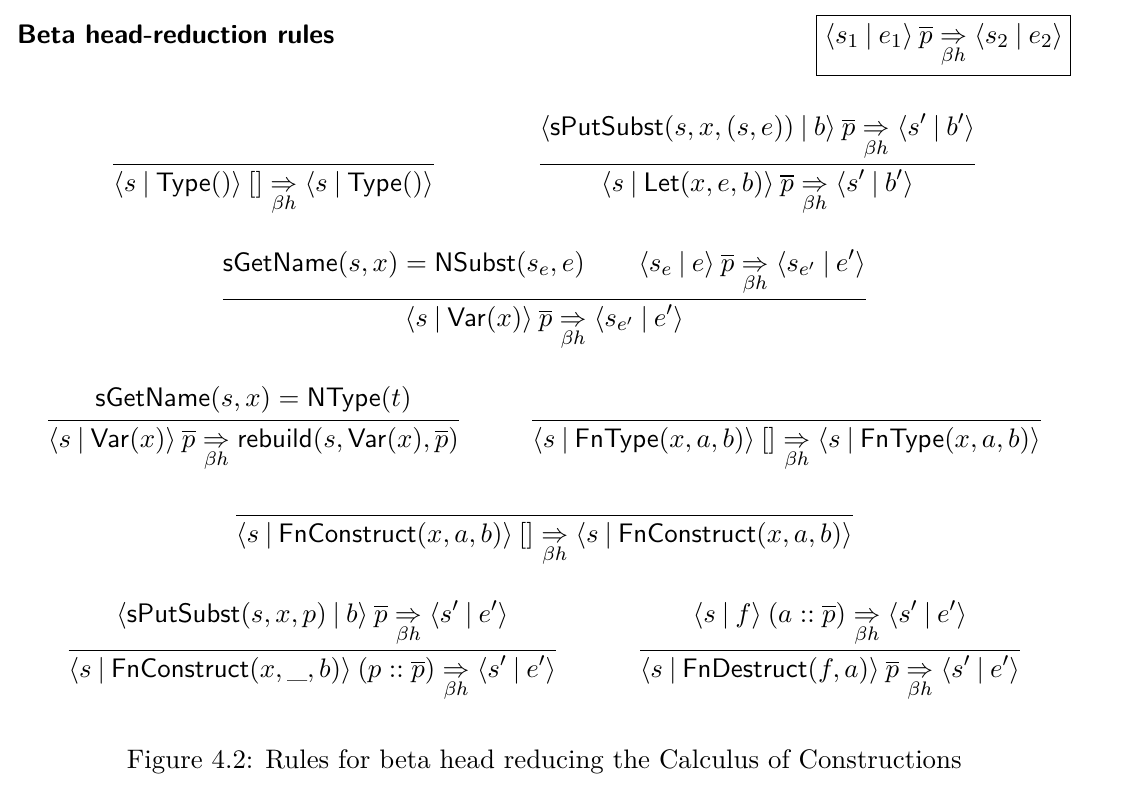
\includegraphics[width=0.5\linewidth]{img/screenshot001}
		\label{fig:screenshot001}
	\end{figure}
	\begin{figure}
		\centering
		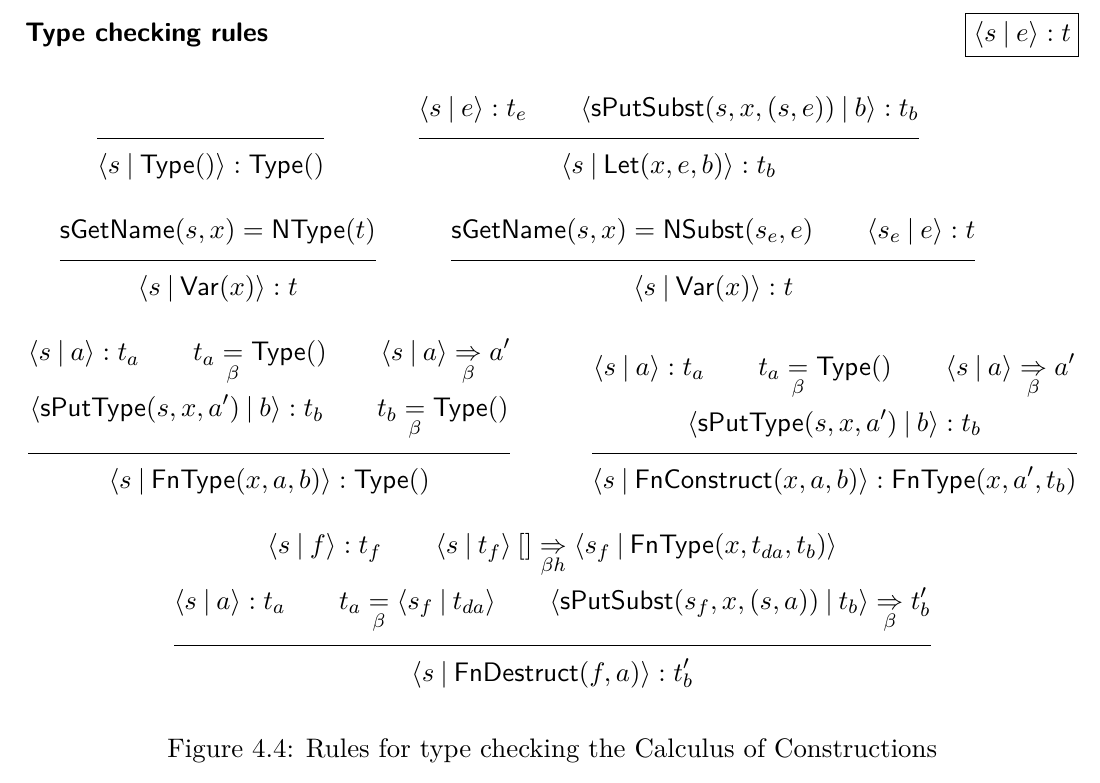
\includegraphics[width=0.5\linewidth]{img/screenshot002}
		\label{fig:screenshot002}
	\end{figure}
	
\end{frame}

\begin{frame}[fragile]{Extra contributions}
	% Refer to thesis for this
Features
\begin{enumerate}
	\item Implemented Inference
	\item Implemented Inductive Data Types
	\item Implemented Universes
	\item Interpreter
	\item Compiler to Clojure
\end{enumerate}
Evaluation
\begin{enumerate}
	\item Comparison with implementation in Haskell
	\item Comparison with implementation in LambdaPi
	\item Evaluation of Spoofax
\end{enumerate}
\end{frame}

\begin{frame}[fragile]{Conclusions}
	Spoofax is a great tool for developing dependently typed languages!\footnote{But there is still room for improvement}
	
	- using scopes as env+context 
	todo beperkingen noemen 
	- statix enforces syntactic uniqueness of metavariable solutions but dependently typed languages use a weaker notion of equality 
	- full thesis coming soonTM
\end{frame}

% block
% exampleblock
% alertblock

\end{document}

